\documentclass[letterpaper,12pt]{article}
\usepackage[spanish]{babel}
\spanishdecimal{.}
\selectlanguage{spanish}
\usepackage[spanish,onelanguage,ruled]{algorithm2e}
\usepackage[utf8]{inputenc}
\usepackage{graphicx}
\usepackage{caption}
\usepackage{subcaption}
\usepackage[top=2cm, bottom=2cm, left=2cm, right=2cm]{geometry}
\usepackage{hyperref}
\usepackage{verbatim}
\usepackage{amssymb}
\usepackage{mathtools}
\newcommand\ddfrac[2]{\frac{\displaystyle #1}{\displaystyle #2}}

\title{Práctica 4  \\ Planeación de rutas utilizando A* y celdas de ocupación}
\author{Laboratorio de Bio-Robótica}
\date{Robots Móviles y Agentes Inteligentes}
\begin{document}
\renewcommand{\tablename}{Tabla}
\maketitle
\section*{Objetivos}
\begin{itemize}
\item Familiarizar al alumno con el uso de mapas de celdas de ocupación.
\item Calcular una ruta a partir de un mapa de celdas de ocupación utilizando el algoritmo A*.
\item Publicar la ruta en un tópico y desplegarla en el visualizador \texttt{rviz}.
\end{itemize}

\section{Introducción: el algoritmo A*}
La planeación de rutas consiste en la obtención de un movimiento continuo libre de colisiones que conecte una configuración inicial, con una final. Se asume que se dispone de una representación del ambiente con información sobre el espacio navegable y el ocupado por los obstáculos. En esta práctica se considera que el robot sólo se mueve sobre un plano y que se tiene una representación que consiste en un mapa de celdas de ocupación (obtenido en la práctica 3). 

Una posible solución es aplicar un algoritmo de búsqueda en grafos. En el caso de las celdas de ocupación, cada celda representa un nodo en el grafo y se considera que está conectada únicamente con aquellas celdas vecinas que pertenezcan al espacio libre. Para determinar los nodos vecinos se puede utilizar conectividad cuatro u ocho. En esta práctica se utilizará la conectivad cuatro. 

A* es un algoritmo de búsqueda que explora la ruta con el menor costo esperado. Para un nodo $n$, el costo esperado $f(n)$ se calcula como 
\[f(n) = g(n) + h(n)\]
donde $g(n)$ es el costo de la ruta desde el nodo origen hasta el nodo $n$ y $h(n)$ es una heurística que determina \textit{un} costo que se esperaría tener desde el mismo nodo $n$ hasta el nodo objetivo. Este costo esperado de hecho subestima el valor real, es decir, se debe cumplir que $h(n) \leq g(n)\quad \forall\; n \in\; Grafo$. 

En la búsqueda por A* se manejan dos conjuntos principales: la \textit{lista abierta} y la \textit{lista cerrada}. La lista abierta contiene todos los nodos que han sido visitados pero no expandidos y la cerrada, aquellos que han sido visitados \textit{y} expandidos (también llamados nodos conocidos). El algoritmo \ref{alg:AStar} muestra los pasos en pseudocódigo para implementar A*. 

\begin{algorithm}
\DontPrintSemicolon
\KwData{Grafo, nodo inicial, nodo meta}
\KwResult{Ruta óptima expresada como una secuencia de nodos}
Cerrado $\leftarrow \emptyset$\;
Abierto $\leftarrow$ \{nodo\_inicial\}\;
previo(nodo\_inicial) $\leftarrow \varnothing$\;
\While{ Abierto $\neq\emptyset$ }
{
  nodo\_actual $\leftarrow$ nodo con el menor valor $f$ del conjunto $Abierto$\;
  Abierto $\leftarrow$ Abierto - \{nodo\_actual\}\;
  Cerrado $\leftarrow$ Cerrado $\cup$ \{nodo\_actual\}\;
  \If{nodo\_actual es nodo\_meta}
  {
    Anunciar éxito y salir de este ciclo\;
  }
  \ForEach{nodo\_vecino de nodo\_actual}
  {
    \textit{//Los nodos vecinos se obtienen con conectividad cuatro}\;
    \If{nodo\_vecino $\in$ Cerrado}{Continuar con el siguiente nodo\_vecino}
    \eIf{nodo\_vecino $\in$ Abierto}
    {
      costo\_temporal $\leftarrow g(\textrm{nodo\_actual}) + d(\textrm{nodo\_actual, nodo\_vecino})$\;
      \If{costo\_temporal $<$ g(nodo\_vecino)}
      {
        $g(\textrm{nodo\_vecino})\leftarrow$ costo\_temporal\;
        $f(\textrm{nodo\_vecino})\leftarrow$ costo\_temporal + heurística(nodo\_vecino, nodo\_meta)\;
        previo(nodo\_vecino) $\leftarrow$ nodo\_actual\;
      }
    }
    {
      $g(\textrm{nodo\_vecino})\leftarrow g(\textrm{nodo\_actual}) + d(\textrm{nodo\_actual, nodo\_vecino})$\;
      $f(\textrm{nodo\_vecino})\leftarrow g\textrm{nodo\_vecino})$  + heurística(nodo\_vecino, nodo\_meta)\;
      previo(nodo\_vecino) $\leftarrow$ nodo\_actual\;
      Abierto $\leftarrow$ Abierto $\cup$ \{nodo\_vecino\}\; 
    }
  }
}
\eIf{nodo\_actual $\neq$ nodo\_meta}
{
  Anunciar falla\;
}
{
  RutaOptima $\leftarrow\emptyset$ \;
  \While{nodo\_actual $\neq\varnothing$ }
  {
    \textit{//El nodo actual se inserta al principio de la ruta}\;
    RutaÓptima $\leftarrow$ \{nodo\_actual\} $\cup$ RutaÓptima \;
    nodo\_actual $\leftarrow$ previo(nodo\_actual)\;
  }
  Regresar RutaÓptima
}
\caption{Búsqueda con A*}
\label{alg:AStar}
\end{algorithm}

El valor $g$ asociado a cada nodo $n$ representa el costo para llegar a $n$ desde el nodo inicial. Como se puede observar en el algoritmo \ref{alg:AStar}, dicho costo se calcula a partir de la distancia $d(n_1,n_2)$ entre dos nodos. Como primera aproximación se puede utilizar la distancia euclidiana, sin embargo, dado que se está trabajando con celdas de ocupación y se emplea conectividad cuatro, la distancia se puede calcular como un entero que incrementa su valor en uno con respecto al nodo anterior.

La heurística $h(nodo_{vecino}, nodo_{meta})$ también puede calcularse mediante distancia euclidiana, sin embargo, dado que se usa conectividad cuatro, el costo computacional se reduce si se emplea \textit{Distancia de Manhattan} y dicha distancia se expresa en número de celdas. 

\section{Desarrollo}

\subsection{Prerrequisitos}
Antes de continuar, actualice el repositorio y recompile:
\begin{verbatim}
   cd ~/RoboticsCourses
   git pull origin master
   cd catkin_ws
   catkin_make
\end{verbatim}

Con el objetivo de facilitar las pruebas, se ha incluido un paquete llamado \texttt{navig\_msgs} que contiene un servicio llamado \texttt{CalculatePath}. El archivo se encuentra en \texttt{navig\_msgs/srv} y tiene el siguinte contenido:
\begin{verbatim}
   geometry_msgs/Pose start_pose
   geometry_msgs/Pose goal_pose
   nav_msgs/OccupancyGrid map
   ---
   nav_msgs/Path path
\end{verbatim}
Como se muestra en el algoritmo \ref{alg:AStar}, los datos de entrada para A* constan de un grafo, un nodo inicial y uno final. Como resultado se obtiene una secuencia de nodos que representan la ruta óptima. El servicio \texttt{CalculatePath} contiene todos los datos necesarios para ejecutar A*, sólo es necesario traducir las posiciones en coordenadas métricas a índices en el conjunto de celdas de ocupación y viceversa. 

El paquete \texttt{map\_server} contiene un nodo del mismo nombre que publica periódicamente un mapa de celdas de ocupación y atiende un servicio con el que se puede obtener dicho mapa. Este nodo recibe por parámetro el nombre del archivo \texttt{.yaml} que contiene la información sobre el mapa a utilizar, en este caso, \texttt{biorobotics\_lab.yaml} (o bien el nombre del mapa construido en la práctica 3). 

Para facilitar el llamado del servicio \texttt{navig\_msgs/CalculatePath} se ha incluido una interfaz gráfica que se encuentra en \texttt{catkin\_ws/src/hri/justina\_simple\_gui}. La figura \ref{fig:gui} muestra una captura de pantalla de ella. Cuando se presiona \texttt{enter} en alguno de los campos del cuadro \textit{Mobile base and navigation}, este programa llama al servicio de nombre \texttt{/navigation/a\_star} de tipo \texttt{navig\_msgs/CalculatePath} con los datos correspondientes en la parte de la petición (\texttt{start\_pose, goal\_pose} y \texttt{map}).
\begin{figure}
\centering
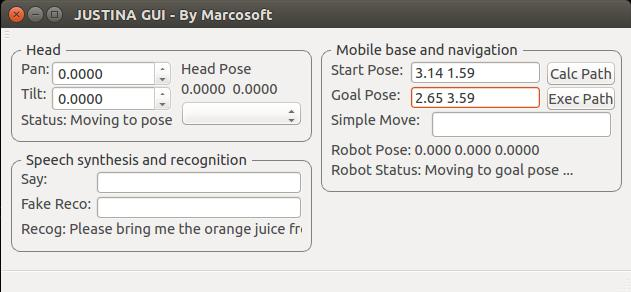
\includegraphics[width=0.65\textwidth]{Figures/gui.jpg}
\caption{Interfaz gráfica}
\label{fig:gui}
\end{figure}

Para correr todos los nodos necesarios (\texttt{map\_server, justina\_simple\_gui}, etc.) ejecute el comando
\begin{verbatim}
   roslaunch bring_up hardware_simul.launch
\end{verbatim}

\subsection{Nodo que calcula y publica la ruta}
Cree un nuevo paquete de ROS con el nombre \texttt{path\_calculator} que tenga las siguientes características:
\begin{itemize}
\item Atender un servicio con el nombre \texttt{/navigation/a\_star}, de tipo \texttt{navig\_msgs/CalculatePath}, que calcule una ruta a partir de un mapa y posiciones inicial y final. 
\item El valor de retorno del servicio (\textit{true, false}) debe corresponder al éxito al calcular la ruta resultante y ésta debe asignarse a la parte de la respuesta (\textit{CalculatePath::Response}) del servicio.
\item El nodo debe publicar de manera periódica la última ruta calculada. El nombre del tópico debe ser \texttt{/navigation/a\_star\_path} de tipo \texttt{/nav\_msgs/Path}. Esto con el objetivo de poder desplegar la ruta calculada en el visualizador \textit{rviz}.
\item Todos los algoritmos deben estar contenidos en funciones o métodos bien definidos. No debe haber \textit{código espagueti}.
\end{itemize}

La figura \ref{fig:path} muestra un ejemplo del resultado esperado en \texttt{rviz}.
\begin{figure}
\centering
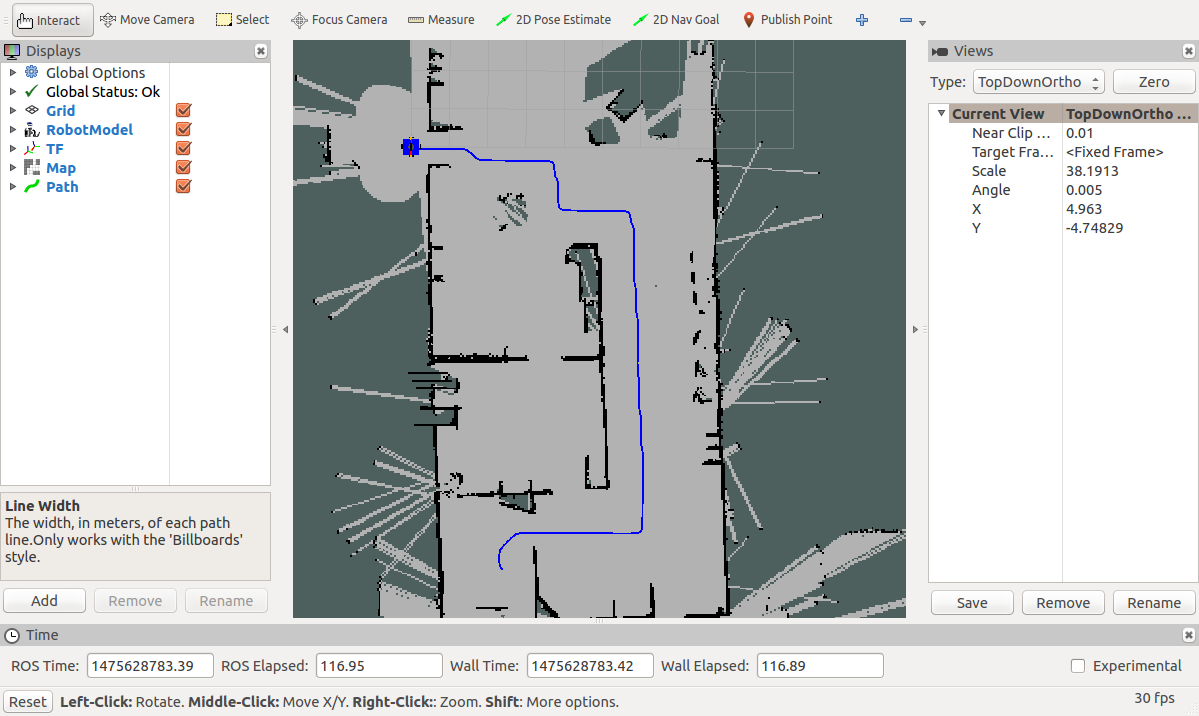
\includegraphics[width=0.9\textwidth]{Figures/Path.png}
\caption{Ejemplo de ruta calculada}
\label{fig:path}
\end{figure}

\section{Evaluación}
\begin{itemize}
\item El cálculo debe ser rápido (retardo no perceptible para un humano). 
\item El programa debe verificar que  inicio y meta NO estén en el espacio ocupado.
\item Se probabará con varios pares de posiciones iniciales y finales aleatorias.
\item Las posiciones iniciales y finales se deben poder cambiar en tiempo de ejecución y se fijarán haciendo uso de la GUI.
\item El código debe estar ordenado.
\item \textbf{Importante: } Si el alumno no conoce su código, NO se contará la práctica.
\end{itemize}

\end{document}
